%% Template.tex; Solar Physics
%% 
\documentclass[namedreferences]{solarphysics}
%
% spr-sola-addons available options:
%  natbib        -- For citations: redefine \cite commands (loads natbib.sty)
%  solaenum      -- makes enumerated list with italics-roman numerals and a single right-bracket
%  solaromanenum -- makes enumerated list with roman numerals and a single right-bracket
%  linksfromyear -- puts a link on a year citation (hyperref must be loaded)
%  optionalrh    -- for optional running title/author
%
\usepackage[optionalrh,solaromanenum]{spr-sola-addons} % For Solar Physics 
%\usepackage{epsfig}                     % For eps figures, old commands
\usepackage{graphicx}                    % For eps figures, newer & more powerfull
%\usepackage{courier}                    % Change the \texttt command to courier style
%\usepackage{amssymb}                    % useful mathematical symbols
\usepackage{color}                       % For color text: \color command
\usepackage{url}                         % For breaking URLs easily trough lines
\def\UrlFont{\sf}                        % define the fonts for the URLs


%% Local definitions
%% please place your own definitions here and don't use \def but
%% \newcommand{}{} or 
%% \renewcommand{}{} if it is already defined in LaTeX
\newcommand{\solphys}{{\it Solar Physics}}
\newcommand{\aap}{    {\it Astronomy \& Astrophysics}}
\newcommand{\aaps}{   {\it Astronomy \& Astrophysics Supplemental}}
\newcommand{\apj}{    {\it Astrophysical Journal}}
\newcommand{\apjl}{    {\it Astrophysical Journal Letters}}
\newcommand{\jgr}{    {\it Journal of Geophysical Research}}
\newcommand{\aapr}{    {\it Astronomy \& Astrophysics Review}}
\newcommand{\grl}{    {\it Geophysical Research Letters}}
\newcommand{\lrsp}{    {\it Living Rev. Solar Phys.}}



%%%%%%%%%%%%%%%%%%%%%%%%%%%%%%%%%%%%%%%%%%%%%%%%%%%%%%%%%%%%%%%%%%
\begin{document}

\begin{article}

\begin{opening}

\title{Investigating the `double eruption' of the 8 March 2011 CME using the \emph{PROBA2}/SWAP imager via advanced image processing methods}

%%%%%%%%%%%%%%%%%%%%%%%%%%%%%%%%%%%%%%%%%%%%%%%%%%%
%% Authors Names
%
\author{J.P.~\surname{Byrne}$^{1}$\sep
        et al.
%        I.~\surname{}$^{2}$      
       }

%%%%%%%%%%%%%%%%%%%%%%%%%%%%%%%%%%%%%%%%%%%%%%%%%%%
%% Runningheads
%
\runningauthor{Byrne et al.}
\runningtitle{SWAP}


%%%%%%%%%%%%%%%%%%%%%%%%%%%%%%%%%%%%%%%%%%%%%%%%%%%
%% Affilations 
%
  \institute{$^{1}$ Institute for Astronomy, University of Hawai'i, 2680 Woodlawn Drive, Honolulu, HI 96822, USA.
                     email: \url{jbyrne@ifa.hawaii.edu} %email: \url{e.mail-b}%\\ 
%             $^{2}$ Second affiliation
%                     email: \url{e.mail-c} \\
             }


%%%%%%%%%%%%%%%%%%%%%%%%%%%%%%%%%%%%%%%%%%%%%%%%%%%
%%% Abstract 
\begin{abstract}
Methods of multiscale image analysis were employed and their efficacy on the SWAP data tested for revealing CME structure while suppressing other features. The methods use successive filtering of an image via a Gaussian and derivative-of-Gaussian produces a number of scales of detail to be inspected. This also produces an image with intensities that represent the relative edge strengths in the original image, which can be used to characterize the structure of interest -- specifically for this case the erupting material involved in the CME. In order to overlap the observations from SWAP and MK4, the core material of the CME in its early eruption phase was chosen for its higher signal to noise ratio than the CME front, for example, that was not discernible in the early stages of the observations. In the LASCO field-of-view, the core material was determined to be moving at the same speed as the CME front, at $\sim500~km~s^{-1}$. The front portion of the core material in the MK4 images was characterized via point-\&-click methodology on the multiscale images of enhanced edges, and an ellipse was fit to the curved front. The same was done for the erupting loop structure observed in SWAP, with the expectation that it might directly correlate to the CME core. However, it was found that the erupting material that starts at the same time and location in both the MK4 and SWAP images, did not proceed to erupt at the same rate. Rather the core material observed in MK4 moves at greater speeds than the loop structures observed in SWAP; rising from an initial speed of $\sim100~km~s^{-1}$ (at $\sim1.5~R_{\odot}$) to a final speed of $\sim400~km~s^{-1}$ (at $\sim2~R_{\odot}$), while the loops continue to steadily rise at $\sim100~km~s^{-1}$. The reason for this is unclear, and requires further investigation.
\end{abstract}



%%%%%%%%%%%%%%%%%%%%%%%%%%%%%%%%%%%%%%%%%%%%%%%%%%%
%% Keywords
%
\keywords{Coronal Mass Ejections, Initiation and Propagation}


\end{opening}
%-------------------------------------------------

%%%%%%%%%%%%%%%%%%%%%%%%%%%%%%%%%%%%%%%%%%%%%%%%%%%
%% Sections
%

\section{Introduction}
\label{intro}

\begin{figure}[ht]
\centering{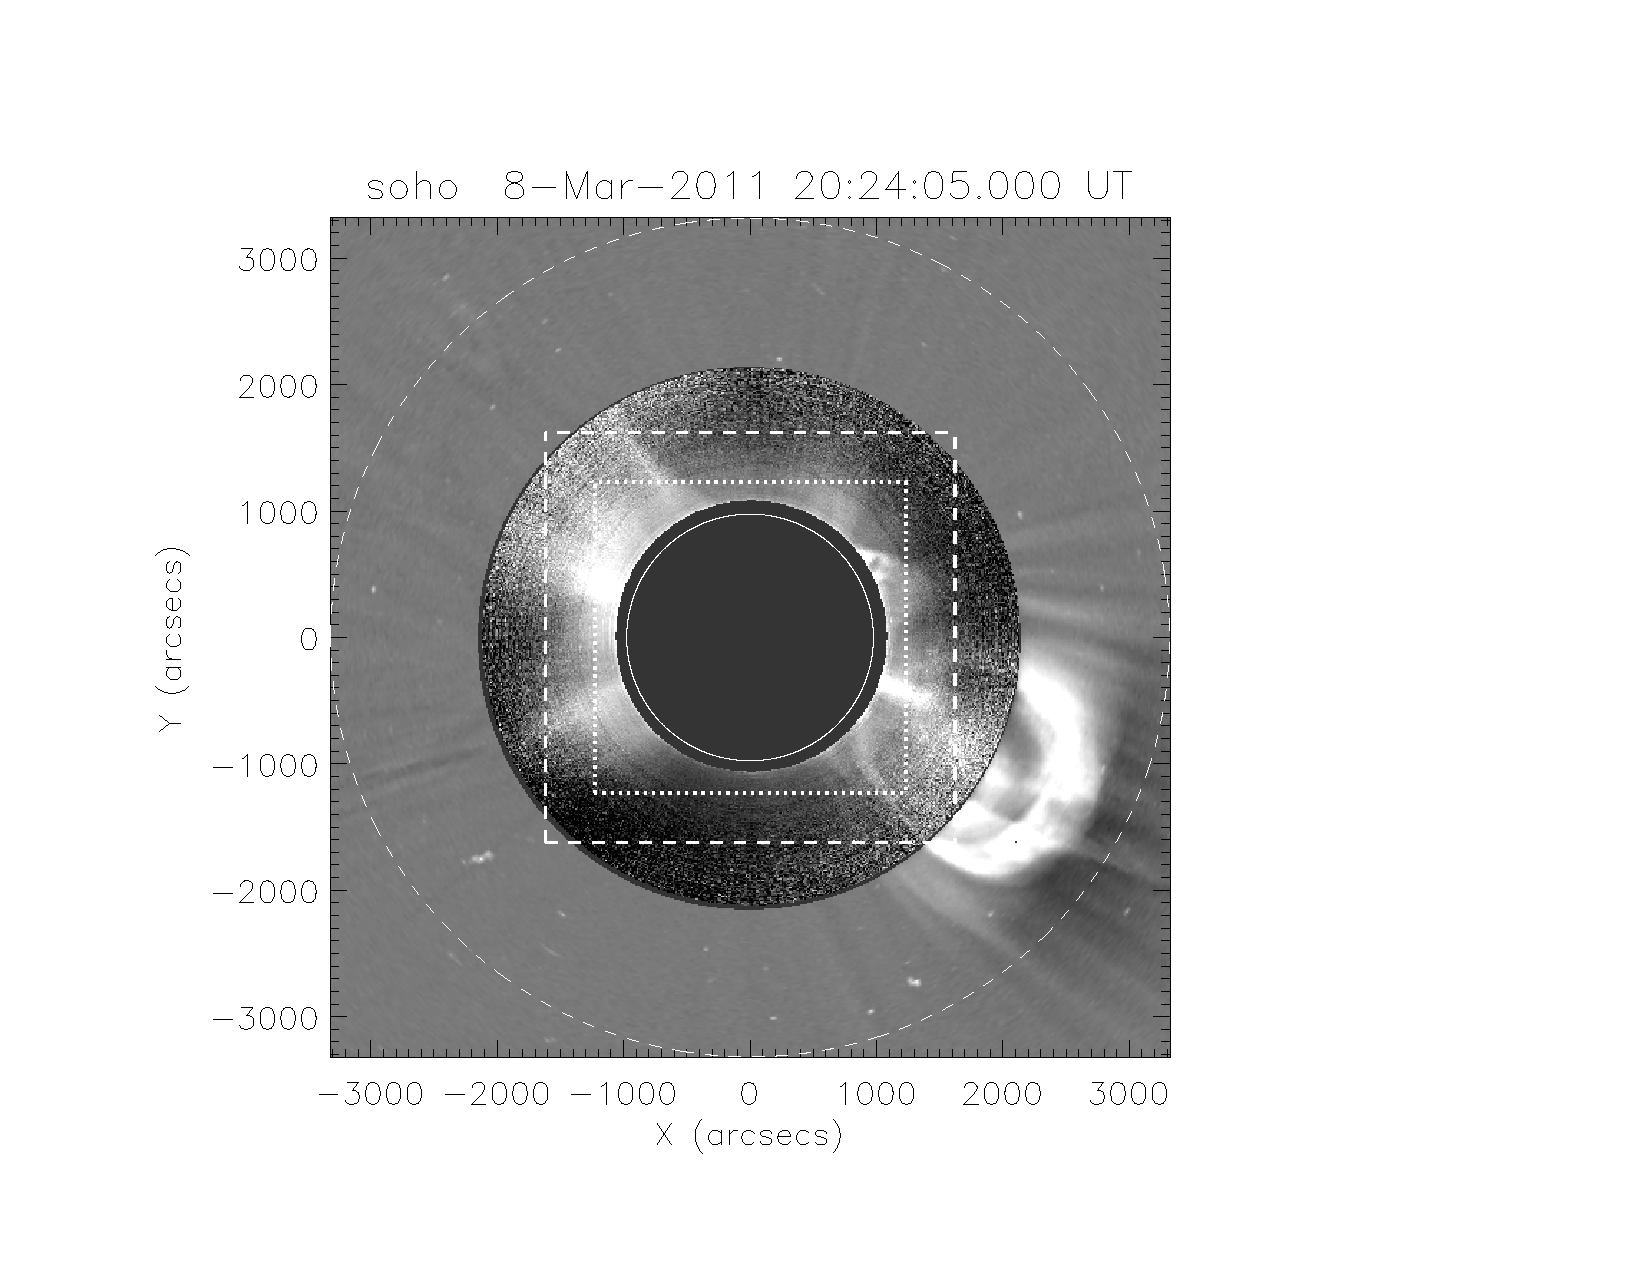
\includegraphics[scale=0.45, trim=60 50 200 70]{images/overlays.pdf}}
\caption{A LASCO/C2 image with an MLSO/MK4 image overlaid in the range 1.1\,--\,2.2~R$_\odot$, dated 2011 March 8 at 20:24 and 20:22~UT respectively. The C2 image has been processed via the CORIMP techniques of normalising radial graded filter (NRGF) and quiescent background subtraction. It has been trimmed to a half-width of 3.4~R$_\odot$, which is the upper limit of the PROBA2/SWAP FOV as indicated by the dashed circle. The SWAP FOV during nominal operations is indicated by the dashed box. The SDO/AIA FOV is indicated by the inner dotted box. The limb of the Sun behind the occulter is indicated by the solid white circle. A CME is observed off the south-west limb as a bright loop structure with some inner core material, as seen here in the Thomson-scattered white-light coronagraph images. It is clear how the SWAP and AIA images can be used to bridge CME observations to the low corona and solar disk, for gaining insight to their initiation phase.}
\label{overlays}
\end{figure}

Coronal mass ejections (CMEs) represent the largest, most dynamic phenomena that originate from the Sun. Propagating at speeds of hundreds up to thousands of kilometers per second \cite{2004JGRA..10907105Y}, the particle densities and energies involved can cause adverse space weather at Earth and elsewhere in the heliosphere \cite{2005AnGeo..23.1033S}. They can lead to geomagnetic storms upon impacting our magneto- sphere, damaging satellites, affecting communication and navigation systems, and increasing the radiation risk for astronauts \cite{2007A&G....48f..11L}. Given their potentially hazardous impact on Earth�s geomagnetic environment, the physics governing their eruption and propagation needs to be understood. 

An important aspect of studying CME initiation, is the ability to resolve their low-corona propagation and associated source regions on the disk: be it a flaring or non-flaring active region, a prominence/filament eruption or other rising loop system, or else a `stealth CME' without any specifically detectable source. Prominence lift-offs often become the core material of a CME, and rising loops often form some part of the CME morphology. Their low-corona kinematics and morphology provide insight into the early forces at play, and so a rigorous study of such phenomena is key to understanding the physics involved.

In order to connect CMEs to their source regions, data from disk imagers such as the Sun Watcher using APS detectors and image Processing (SWAP; \opencite{2013SoPh..286...43S}) onboard the second Projects for Onboard Autonomy (\emph{PROBA2}; \opencite{2013SoPh..286....5S}) and the Atmospheric Imaging Assembly (AIA; \opencite{2012SoPh..275...17L}) onboard the Solar Dynamics Observatory (\emph{SDO}; \opencite{2012SoPh..275....3P}), may be used in tandem with coronagraph observations. However, difficulties in the interpretation of the observed features arise due to the varying instrument specifications, e.g., image passbands, fields-of-view, cadences, etc. Therefore, to bridge the gap between the white-light images of the extended corona and the EUV observations of the solar disk and low corona, the SWAP imager was used in conjunction with the MLSO/MK4 coronagraph to directly compare the observations of CMEs as they erupt through the overlapping fields-of-view (Fig.\,\ref{overlays}). This allows a direct correspondence of features in the EUV images with those in the white-light images, providing new insight into the connection of CMEs to the Sun during their initial phases of eruption and acceleration away from their source regions on the disk.

A difficulty exists in studies of coronal structure that are prone to low signal-to-noise ratios in the observational data. Low-coronal white-light observations using a coronagraph are problematic due to the strong radial brightness gradient and issues with scattered light in the instrument, while extended EUV disk observations are problematic due to the strong drop-off in emission brightness with increasing coronal height. These common issues with solar observational data motivate the development and use of advanced image processing techniques to suppress noise and enhance structures in the image data \cite{2011ApJ...737...88D, 2011AdSpR..47.2118G, 2011igi-global, 2008ApJ...674.1201S, 2008SoPh..248..457Y, 2006SoPh..236..263M, 2003A&A...398.1185S}.


\section{Observations \& Techniques}

Methods of multiscale image processing have been developed in recent years for use on coronagraph images to enhance the underlying structure. The fundamental idea behind these methods is to highlight details apparent on different scales within the data. Therefore, multiscale techniques provide an ability to remove small-scale features in images, essentially suppressing the noise such that the structures of interest can be revealed in greater detail. By applying them to coronagraph images, the morphology of CMEs as they propagate through the corona in a sequence of observations can be determined with better accuracy than previously possible (\opencite{2009A&A...495..325B}, \citeyear{2012ApJ...752..145B}). 

These methods are now demonstrated for use on the MK4 coronagraph and SWAP EUV imager, to provide insight to the low-coronal morphology of erupting structures that may form CMEs. Details on the fundamental technique are outlined in \inlinecite{2008SoPh..248..457Y} wherein the magnitude of the multiscale gradient is used to show the relative strength of the detected edges in the image structure at a particular scale of the multiscale decomposition (i.e., the strongest edges appear brightest). To artificially increase the signal-to-noise ratio of the edge detections even further, the magnitude information from the scales most relevant to the coronal structures of interest may be multiplied together, neglecting the largest scales that smooth out the coronal signal, and the smallest scales that reveal the finer structure and noise (see \opencite{2012ApJ...752..145B} for details). Thus the magnitude of the multiscale gradient across the dominant edges of coronal loops and CMEs is further enhanced for subsequent characterization of their morphology. 

Figure\,\ref{smaps} shows a combined \emph{PROBA2}/SWAP and \emph{SDO}/AIA\,171{\AA} image of an erupting prominence observed at 17:43\,UT on 16\,April\,2012. The multiscale edge enhancement technique is applied and the dominant structures of interest in the prominence become more readily distinguishable in the images, noting the effective noise suppression in the extended SWAP image. (The images are easily combined more smoothly, but the boundary between them is included here for reference.) The strength of this technique for characterizing the prominence structure is shown in Fig.\,\ref{combine_polar_figs}, on the polar-unwrapped SWAP image of the same eruption. A comparison of the signal intensity across the image at height 1.3\,R$_{\odot}$


\begin{figure}[t]
\centering{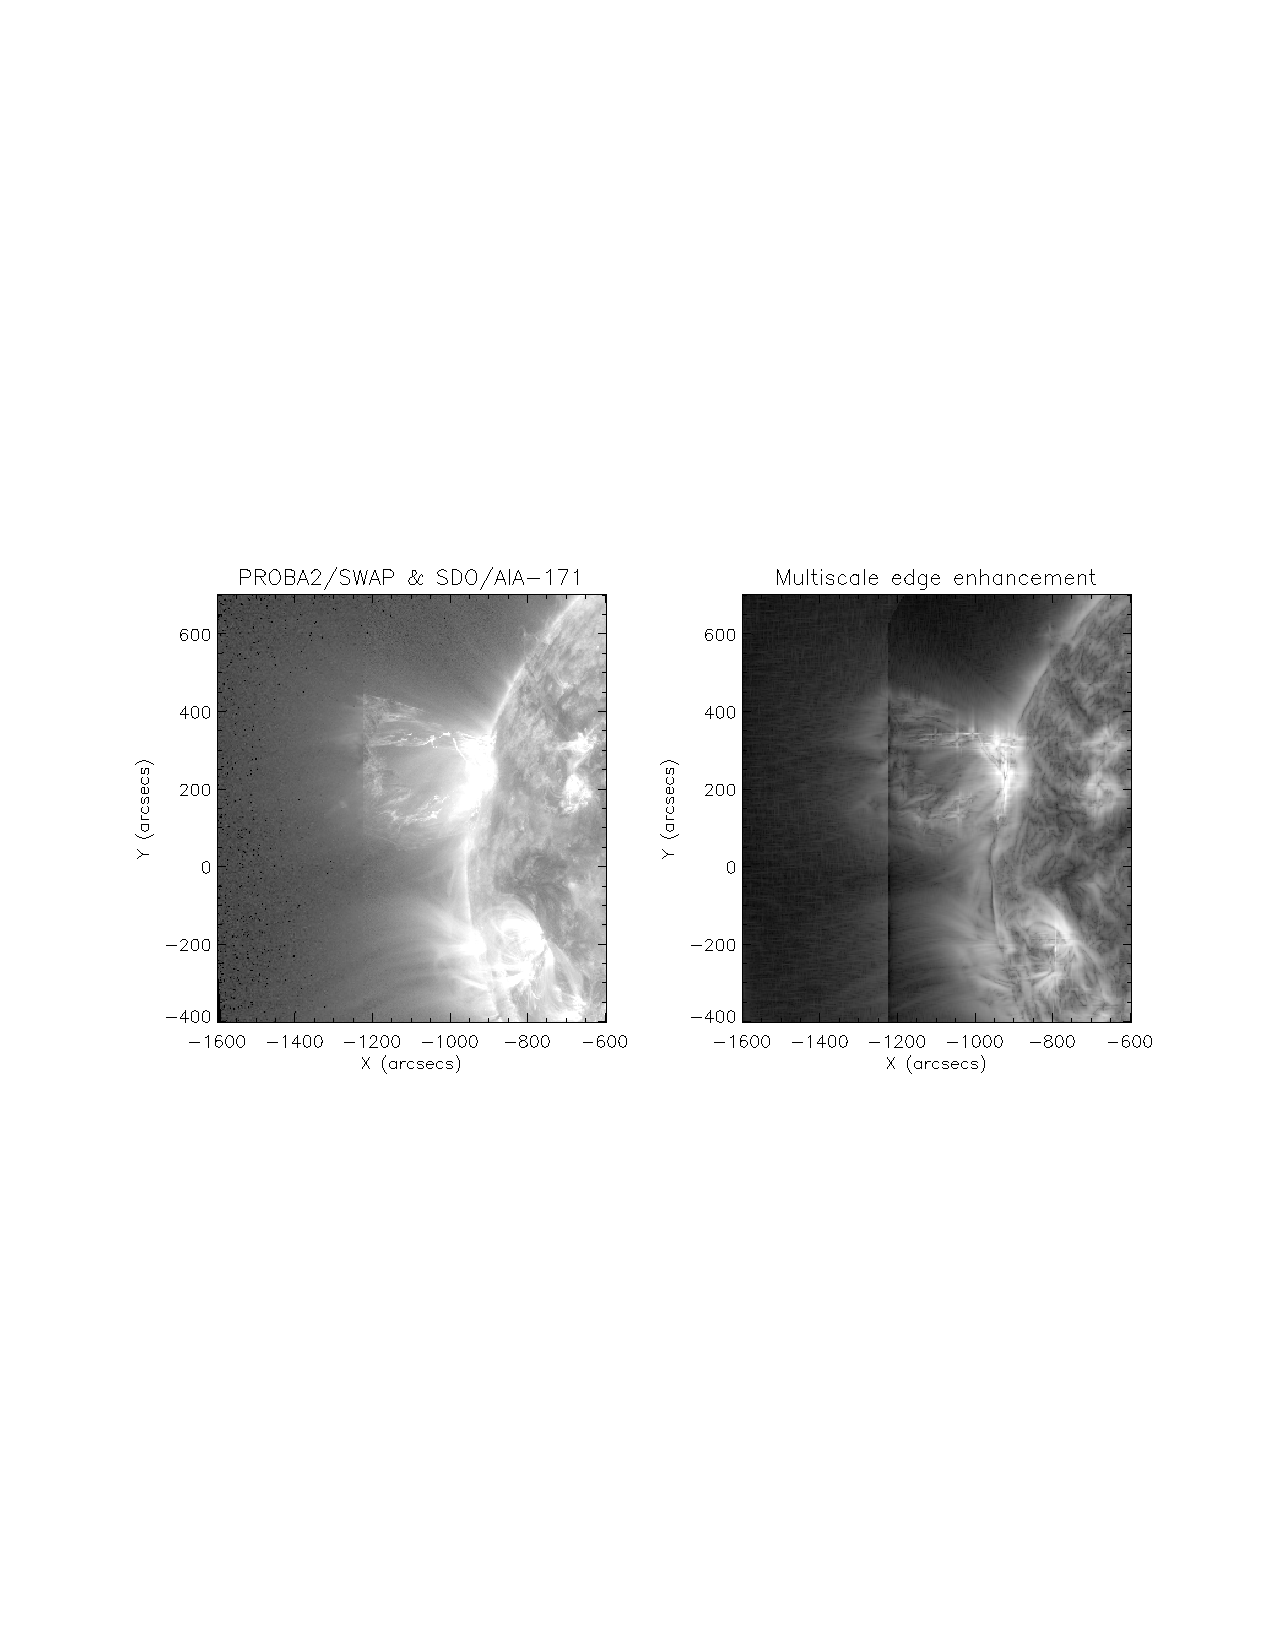
\includegraphics[scale=0.68, trim=65 270 50 250, clip=true]{images/smaps.pdf}}
\caption{Combined PROBA2/SWAP and SDO/AIA-171 image of an erupting prominence observed on 2012 April 16 at 17:43~UT. \emph{Left:} The level-1 data, with the AIA image extending to approximately 1.3~R$_\odot$ and SWAP continuing out to $\sim$\,1.7~R$_\odot$. \emph{Right:} The result of a multiscale edge enhancement technique: the intensity showing the relative strengths of the detected edges along the structures in the image. A substantial amount of detail is revealed within the erupting prominence material and across the solar disk and corona.}
\label{smaps}
\end{figure}

\begin{figure}[t]
\centering{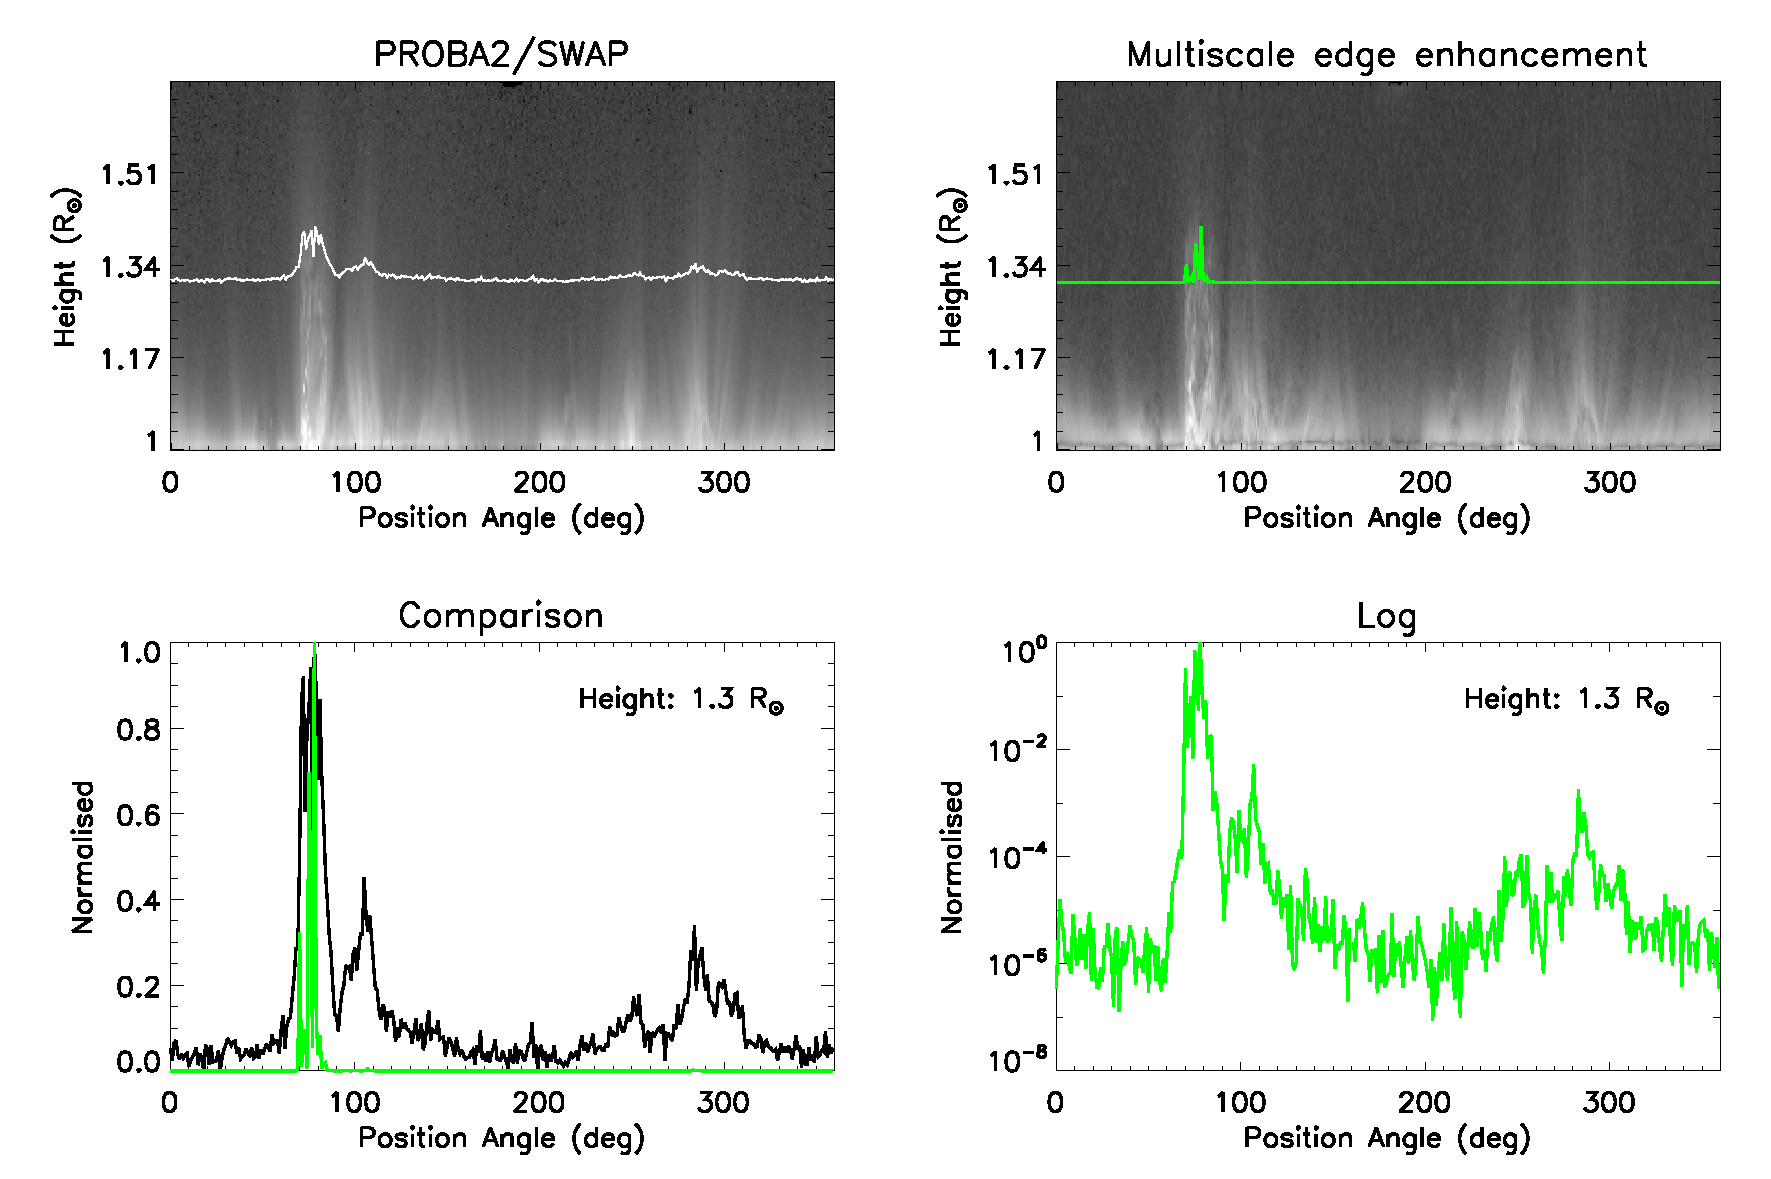
\includegraphics[scale=0.4, trim=0 0 0 0]{images/polar_fig_swap.pdf}}
\caption{The top two panels show polar-unwrapped images of the solar corona across the PROBA2/SWAP FOV on 2012 April 16 at 17:43~UT; left being the level-1 data, right being the enhanced data. Across each image, at a constant height of 1.3~R$_\odot$, an intensity slice is plotted (of arbitrary normalised units) to demonstrate how the background coronal structure is suppressed by the multiscale techniques, to highlight only the complex structure of the prominence. The bottom left plot shows a direct comparison of the two intensity slices, where the prominence is located between 70\,--\,90$^\circ$. The bottom right plot shows a log scale of the normalised intensity slice across the enhanced image to demonstrate that the rest of the coronal structure is still present, just strongly suppressed relative to the prominence material.}
\label{combine_polar_figs}
\end{figure}

\begin{figure}[t]
\centering{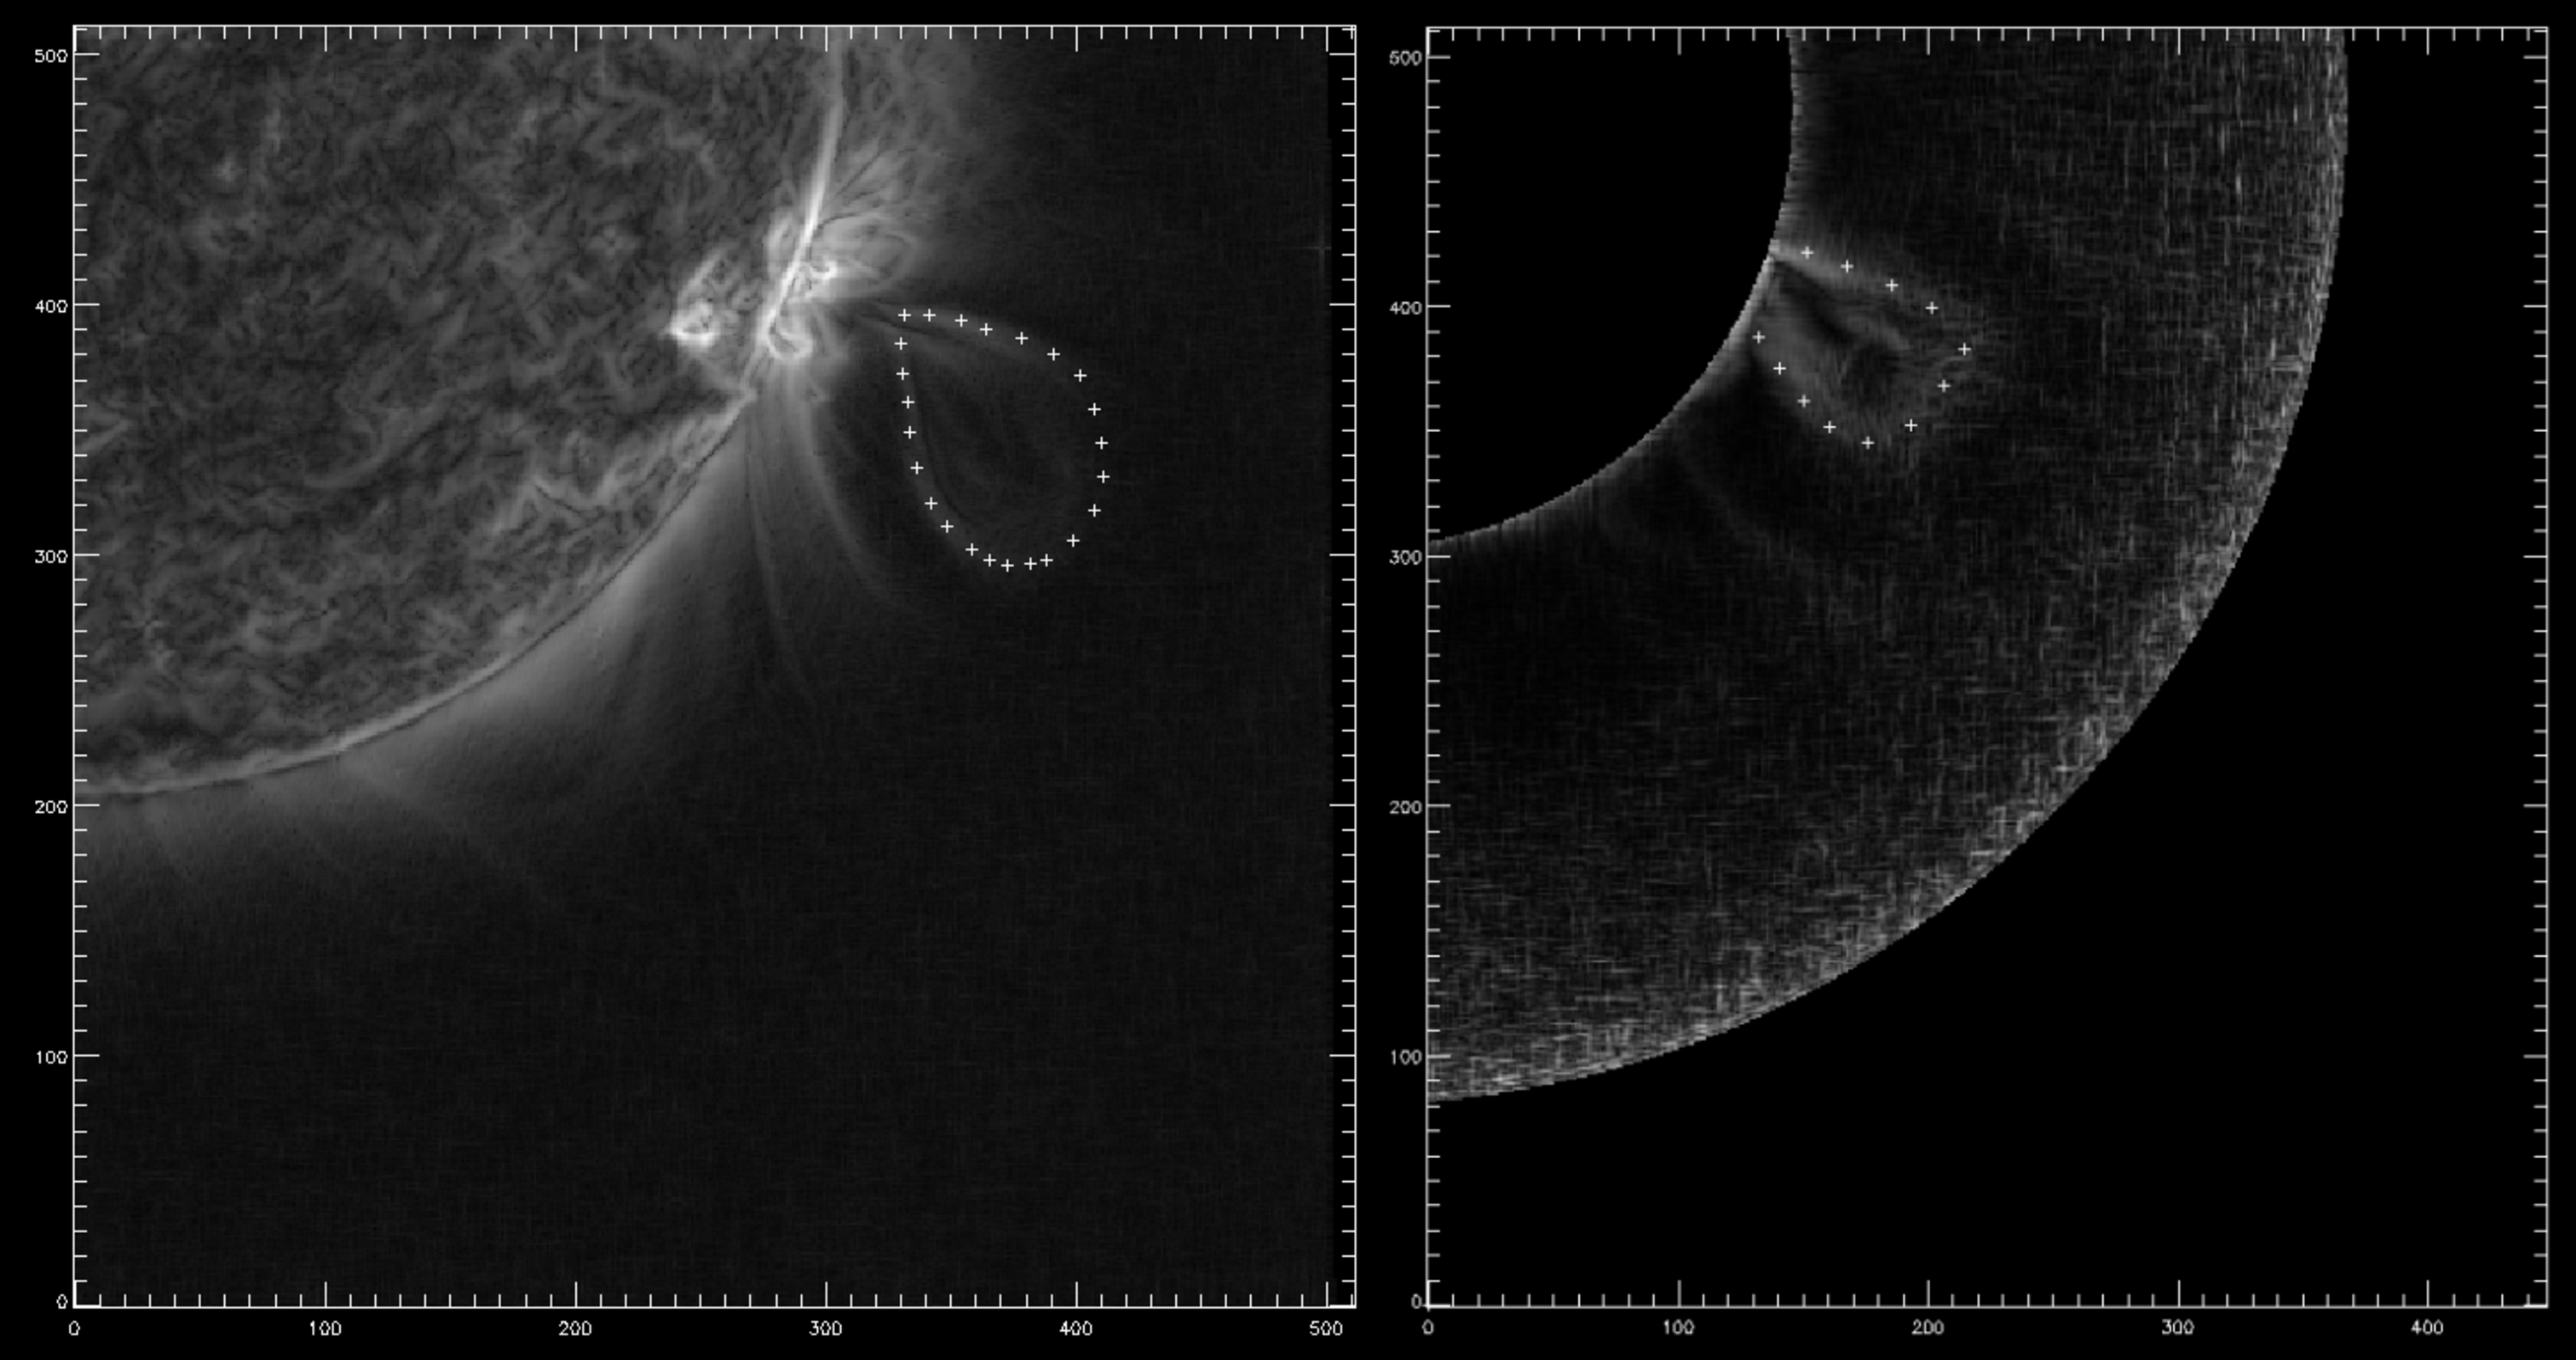
\includegraphics[scale=0.15, trim=0 0 0 0]{images/swap_mk4_temp.pdf}}
\caption{SWAP (left) and MK4 (right) observations of the erupting loop system that forms the inner core of the CME on 2011\,March\,8, at times 19:52 and 19:53\,UT respectively. The images have been processed via the multiscale decomposition, showing here intensities that represent the magnitude of the detected edges, at a particular scale with high signal-to-noise ratio.}
\label{swap_front}
\end{figure}

\begin{figure}[t]
\centering{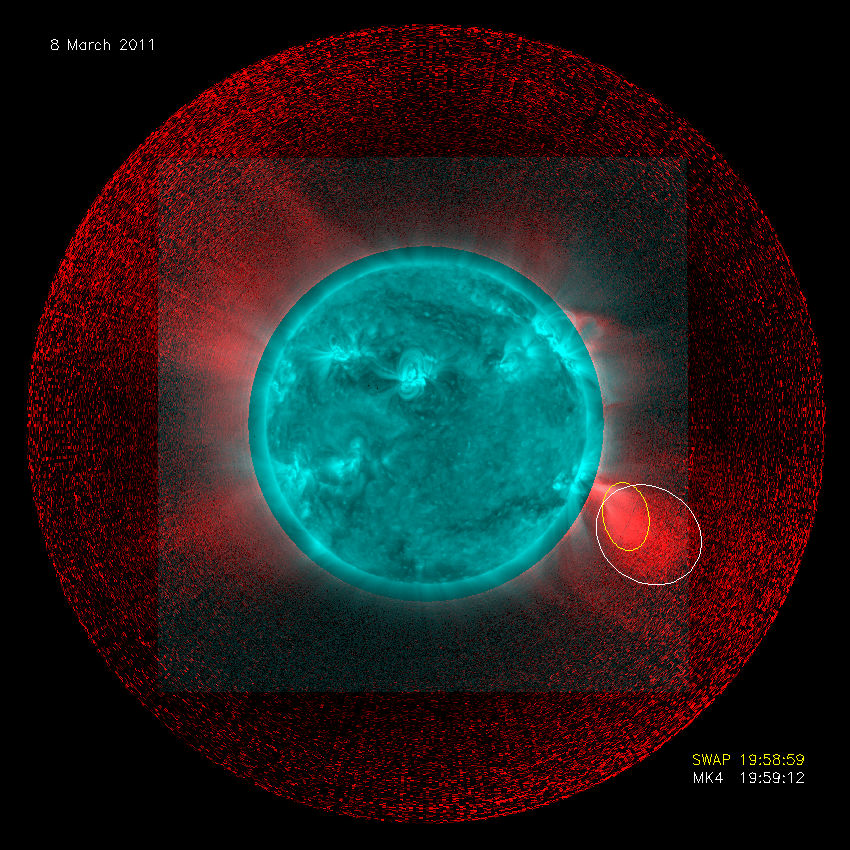
\includegraphics[scale=0.3, clip=true, trim=60 0 0 0]{images/combined.eps}}
\caption{A merged SWAP (blue) and MK4 (red) image with the ellipse fits to the characterized CME core material as observed by each instrument.}
\label{mk4_swap_fig}
\end{figure}

\begin{figure}[t]
\centering{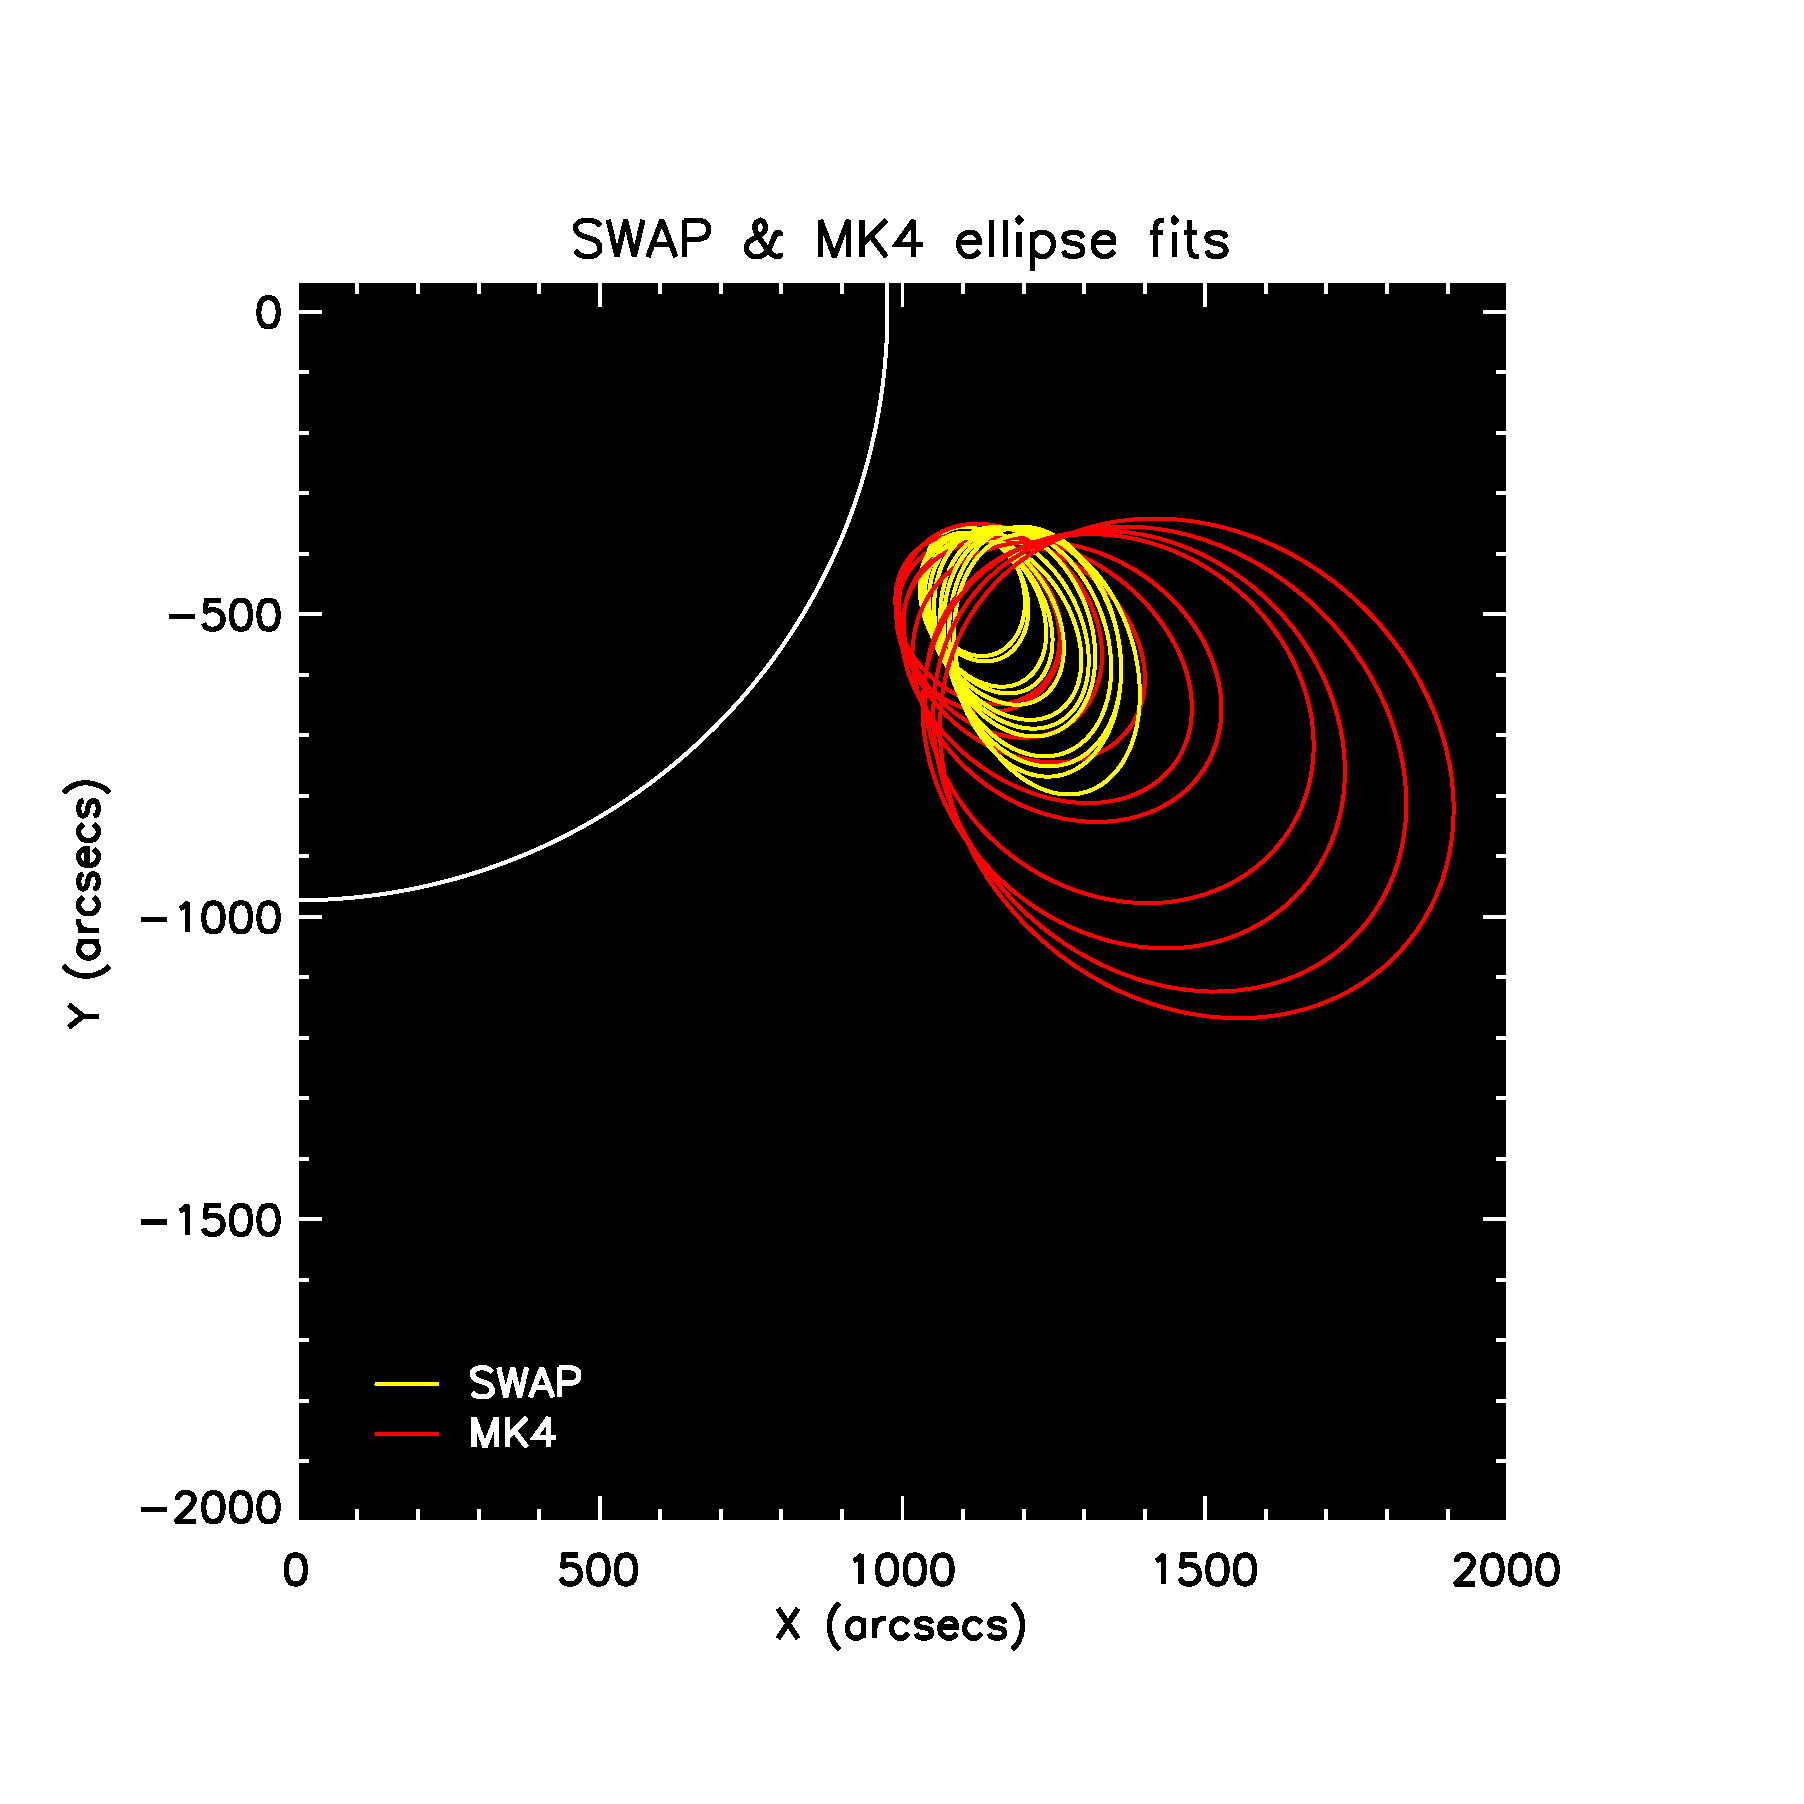
\includegraphics[scale=0.3, clip=true, trim=0 65 110 90]{images/ells_fig.eps}}
\caption{The SWAP and MK4 ellipse fits to the characterized CME core material over the course of the eruption.}
\label{mk4_swap_ells}
\end{figure}

\section{`Double Eruption' of the 8 March 2011 CME}

A CME erupted from active region NOAA\,11165 (S20W91) at approximately 19:30\,UT on 8\,March\,2011. The active region caused numerous flares during its evolution across the disk, notably an M1.5 flare at GOES start-time 19:35\,UT associated with the rising loop system that erupted to form the core material of the CME. The loop system evolution is clearly visible up to $\sim$1.3\,$R_{\odot}$ in \emph{SDO}/AIA (ref) images, with the proceeding eruption observed to a height of $\sim$1.6\,$R_{\odot}$ in the larger field-of-view of the \emph{PROBA2}/SWAP (ref) (17.4\,$nm$) imager.

The CME is observed in MLSO/MK4 (ref) coronagraph data, providing white-light polarization brightness images of the corona from $\sim$1.14\,--\,2.86\,$R_{\odot}$. The data was prepared via an instrumental vignetting function that maximizes the image contrast by offsetting the radial brightness gradient in order to best reveal structures such as CMEs and streamers.

In order to best reveal the eruption material in the low signal-to-noise SWAP and MK4 images, multiscale methods of noise suppression and edge enhancement were employed, as developed by \inlinecite{2008SoPh..248..457Y} and repeatedly shown effective in the analysis of CME morphology \cite{2012ApJ...752..145B,2009A&A...495..325B}. This allowed a point-\&-click characterization of the core material of the CME, which was the brightest structure to be tracked through the different imagers when the CME front was not yet fully formed. The rising loop system observed in the SWAP images, and the erupting CME core material that coincided both temporally and spatially with the rising loops, at least initially, were characterized by ellipse-fits to the detected front edges of the structures. Figure\,\ref{mk4_swap_figs} (left) shows an overlay of a SWAP and MK4 image during the eruption at times 19:58:59 and 19:59:12\,UT respectively, with the ellipses fit to the erupting fronts at those times (from point-\&-click characterizations of the edge enhanced multiscale decompositions of the images). Figure\,\ref{mk4_swap_figs} (right) shows the progression of the ellipse fits to the fronts over the course of the eruption, indicating how the white-light material observed in MK4 propagates away from the source quicker than the EUV material observed in SWAP. These methods were also applied to the \emph{SOHO}/LASCO (ref) observations of the CME, in order to characterize both the dynamical evolution of the CME front and its bright core that was directly associated with the core material observed with MK4.


The CME onset was observed as a series of rising loops, that attained an initial steady height in the low corona, of approximately half a solar radii, before destabilizing and becoming the inner core material of a typical three-part CME that propagated out through the corona at a bulk speed of $\sim$400$\,km\,s^{-1}$, following an initial acceleration of $\sim$20$\,m\,s^{-2}$ away from the sun. The characterized eruption of the CME core in the MK4 images shows this same kinematic profile, however the associated erupting loop structures in the SWAP images proceed at a slower rate, moving at a speed of only $\sim$100$\,km\,s^{-1}$. The different height-time profiles of the SWAP and MK4 observations is shown in Fig.\,\ref{plot_heights_inner}.

\begin{figure}[ht]
\centering{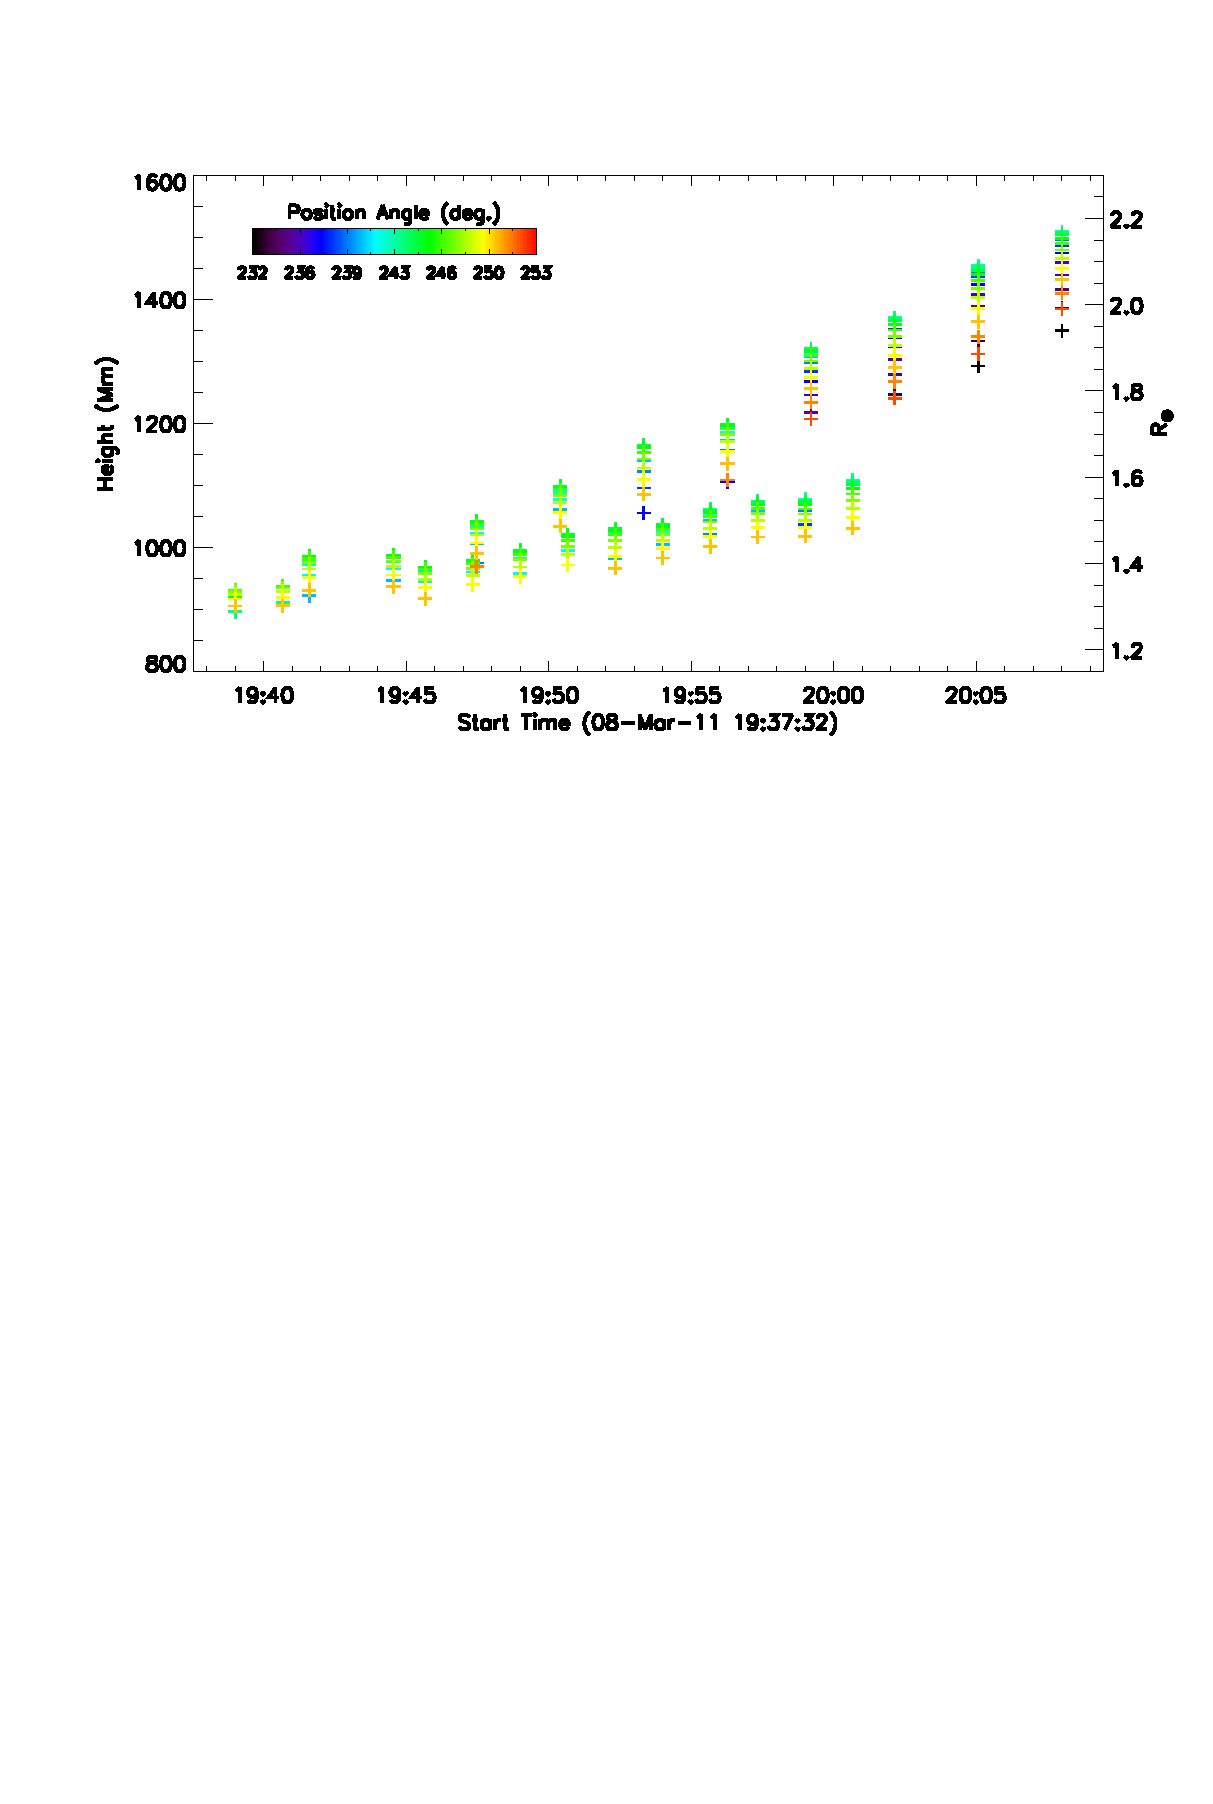
\includegraphics[scale=0.43, trim=30 500 0 70, clip=true]{images/plot_heights_inner.eps}}
\caption{The `double eruption' height-time profile of the characterized eruption observed simultaneously with the SWAP imager and MK4 coronagraph (see the ellipse-fits in Fig.\,\ref{mk4_swap_figs} above). The erupting EUV loops move at a speed of $\sim$100$\,km\,s^{-1}$ while the associated core of the resulting CME is observed to accelerate up to a speed of $\sim$400$\,km\,s^{-1}$.}
\label{plot_heights_inner}
\end{figure}

\begin{figure}[!t]
\centering{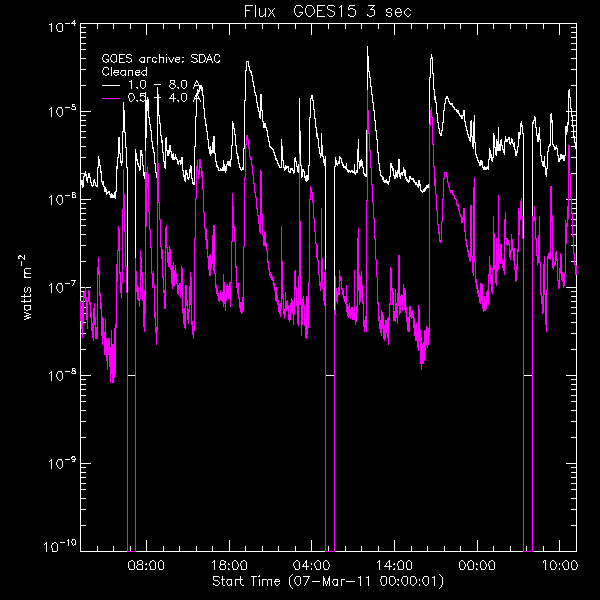
\includegraphics[scale=0.35, trim=0 0 0 0, clip=true]{images/xrayflux.png}}
\caption{GOES x-ray flux.}
\label{xrayflux}
\end{figure}

\begin{figure}[!t]
\centering{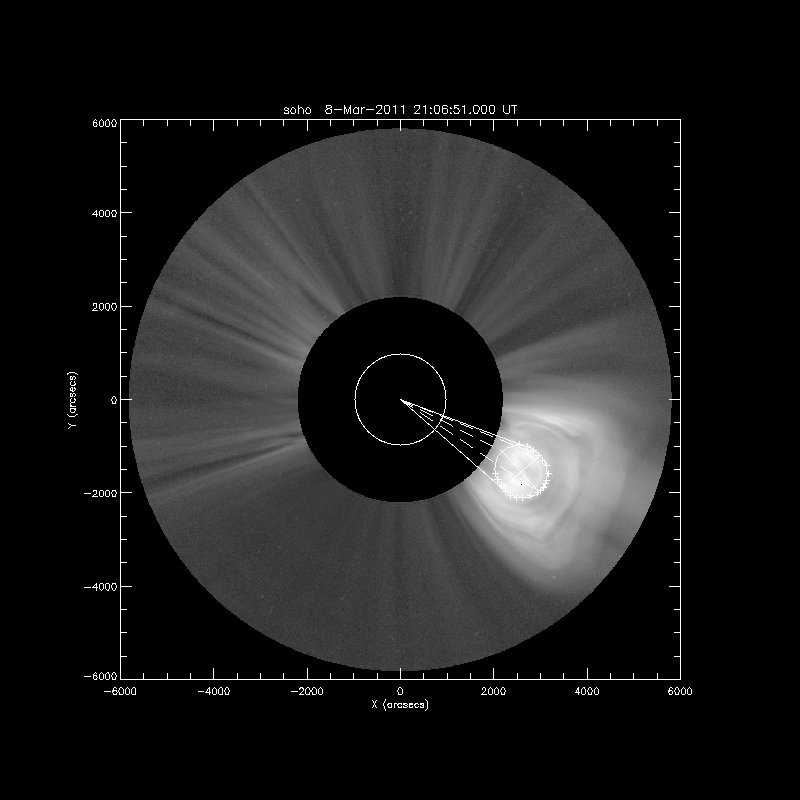
\includegraphics[clip=true, scale=0.32, trim=30 70 70 70]{images/ell_front_c2.png}}
\caption{LASCO/C2 observation of the CME at 21:06~UT on 8 March 2011.}
\label{c2}
\end{figure}

\begin{figure}[!t]
\centering{\includegraphics[clip=true, scale=0.5, trim=0 0 0 0]{images/plot_kins_quartiles_savgol_20110308T190650.eps}}
\caption{LASCO kinematics of the CME on 8 March 2011.}
\label{lasco_kins}
\end{figure}


% \section{}%\label{s:?} 




%% Figure 
%
% \begin{figure} 
% \centerline{\includegraphics[width=0.5\textwidth,clip=]{<fig.eps>}}
% \caption{}%\label{fig:?}
% \end{figure}



%% Table
%
% \begin{table}
% \caption{}%\label{tbl:?}
% \begin{tabular}{}     
% \hline
% \multicolumn{2}{c}{<>}
% <data>
% \hline
% \end{tabular}
% \end{table}
  

%%%%%%%%%%%%%%%%%%%%%%%%%%%%%%%%%%%%%%%%%%%%%%%%%%%%%%%%%%%%%%%%%%%%%%%%%%%
%% Appendix
%
% \appendix   



%%%%%%%%%%%%%%%%%%%%%%%%%%%%%%%%%%%%%%%%%%%%%%%%%%%%%%%%%%%%%%%%%%%%%%%%%%%
%% Acknowledgements
%
 \begin{acks}
 
This work is supported by SHINE grant 0962716 and NASA grants NNX08AJ07G and NNX13AG11G to the Institute for Astronomy.

SWAP is a project of the Centre Spatial de Li`ege and the Royal Observatory of Belgium funded by the Belgian Federal Science Policy Office (BELSPO).

MK4 data is provided courtesy of the Mauna Loa Solar Observatory, operated by the High Altitude Observatory, as part of the National Center for Atmospheric Research (NCAR). NCAR is supported by the National Science Foundation.

%The \emph{SOHO}/LASCO data used here are produced by a consortium of the Naval Research Laboratory (USA), Max-Planck-Institut fuer Aeronomie (Germany), Laboratoire d'Astronomie (France), and the University of Birmingham (UK). SOHO is a project of international cooperation between ESA and NASA. \emph{SDO} data supplied courtesy of the NASA/\emph{SDO} consortia. 

 \end{acks}


%%% %%%%%%%%%%%%%%%%%%%%%%%%%%%%%%%%%%%%%%%%%%%%%%%%%%%%%%%%%%%
%% Bibliography
%
% Using BibTeX
%
 \bibliographystyle{spr-mp-sola.bst}
% %\bibliographystyle{spr-mp-sola-cnd} %% Alternative style: no title, no concluding page
 \bibliography{references.bib}  
%
% Without BibTeX 
% \begin{thebibliography}{}
% \bibitem[\protect\citeauthoryear{Author}{Year}]{key}
%   <bibliographical entry>
%
% \bibitem[\protect\citeauthoryear{}{}]{}
%   
%  
% \end{thebibliography}

\end{article} 
\end{document}
